\section{Implementation}
Lorem ipsum

\subsection{Architecture}

\subsubsection{Wave File Wrapper}
The WaveFileWrapper class is responsible for reading, parsing and validating the wave file. It provides an API for accessing all information need for creating the report. When creating such a wrapper object, an error is thrown when the validation fails at some point. The samples are provieded as an array of arrays. Each element of the outer array represents one sample and the elements of the inner array represent the amplitude of each channel. 

\begin{figure}[H]
    \centering
    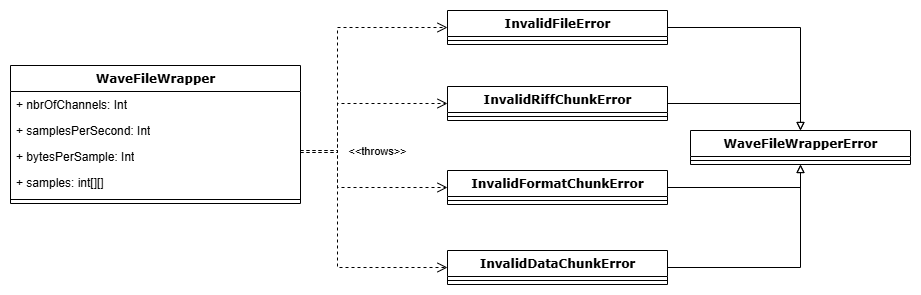
\includegraphics[width=1.0\textwidth]{../assets/wave_file_wrapper.png}
    \caption{WaveFileWrapper class overview}
\end{figure}

\subsection{Processes}
The following diagram shows which steps are involved when creating a noise report from a wave file.

\begin{figure}[H]
    \centering
    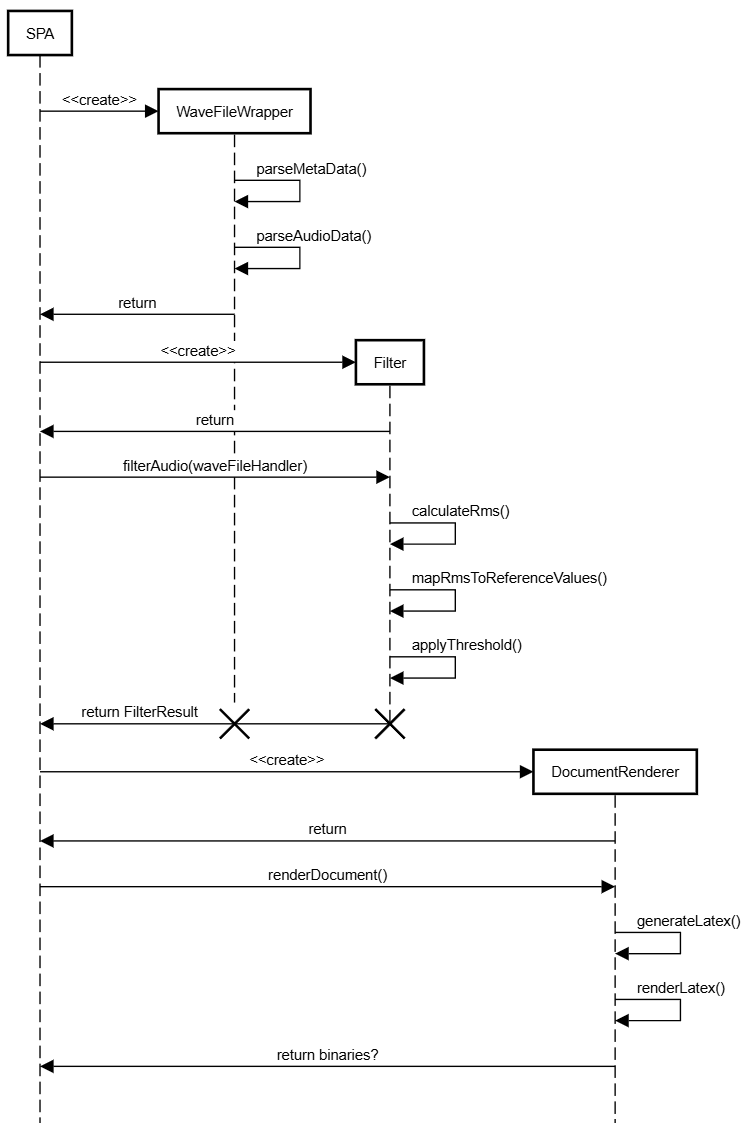
\includegraphics[width=0.8\textwidth]{../assets/sequence_diagram_from_wave_file_to_pdf.png}
    \caption{Sqeuence diagram of steps involved when creating a noise report}
\end{figure}

\subsubsection{Parsing the Wave File}
The WaveFileWrapper class will be responsible for parsing the file. The format itself is straight forward\cite{wav_file_format_wikipedia}, the only importend thing is that the whole file is Little-Endian. It starts with a 12 byte header which we use to verify that the given file is actually a wave file. After the header comes a 24 byte chunk which contains information about the data format. We are interested in the following fields:
\begin{itemize}
    \item AudioFormat (2 bytes): only handle PCM i guess?
    \item NbrChannels (2 bytes): is used to parse individual samples
    \item Frequence (4 bytes): number of samples per second, this is needed for filtering and summarzing 
    \item BitsPerSample (2 bytes): number of bits for a single sample for a single channel, is used to parse individual samples
\end{itemize}
After the format chunk comes an optional list chunk containing some additional metadata in which we are not interested. There we skip that chunk and go straight to the data chunk. This chunk starts with a 4 byte long DataBlocID, which should always have the value 'data'. The next 4 byte represent the number of samples in the data. After that comes the actual audio data. To parse a single sample, we need to parse a frame. A frame contains the data of all channels and has therefore a size of \[\frac{NbrChannels * BitsPerSample}{8}\] bytes. 

\subsubsection{Calculating Decibel Values}
If an audio file consists of several channels, we use the average of the channels as the value of the sample.
When we want to analyse where a certain decibel threshold has been exceeded, we must have accurate values. People only perceive something as loud if it is loud over a longer period of time. Short peaks are perceived less. Therefore, when determining the effective loudness of audio, we do not use the loudness of individual samples, but rather the average of a number of samples over a certain period of time. We will, as usual when working with audio, the root mean squere, as we are interested in the absolute amplitude values.
The calculated average then depends heavily on how long the time period is. In practice, 300ms is usually used\cite{timespan_for_audio_rms_calculate}. This is also the default value, which can be adjusted by the user via the settings.
The decibel value is calculate with the following formula\cite{decibel_wikipedia}:
\[20 * \log_{10} (sample)\] 

As mentioned in the introduction, the audio file only contains relativ values. We therefore need to map the RMS values to the number range of the reference values.
